\chapter{Mitigation Strategies}
\label{chap:mitigationstrats}

\section{Nature-based Solutions for bank erosion}

When it comes to Nature-based solutions, the question arises what this definition means. A quite general definition of nature based solutions would be;

\textit{“Nature-based Solutions are actions to protect, conserve, restore, sustainably
use and manage natural or modified terrestrial, freshwater, coastal and marine
ecosystems, which address social, economic and environmental challenges
effectively and adaptively, while simultaneously providing human well-being,
ecosystem services, resilience and biodiversity benefits” (United Nations, 2022,
p. 2)}

Although this definition may give a thought that it only concerns natural and biodiversity increasing ideas this is actually not the case. For example the impact of NBS on the local economies and communities is of an equal importance. When it comes to weighing the different NBS against each other this report will make use of the seven goals of the IUCN which must be achieved as good as possible. The seven goals are presented below;

\begin{figure}[H]
    \centering
    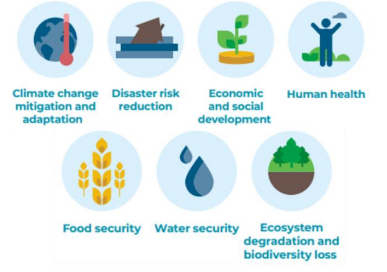
\includegraphics[width=0.50\linewidth]{figures/ThesevenNBSgoals.png}
    \caption{Seven goals for achieving a good NBS}
    \label{fig:placeholder}
\end{figure}

\subsection{Resistance against NBS}

Although NBS are widely known in the scientific world, most people have never heard of these solutions. So, when implementing a solution which can't be described as a classical solution, there is a big change of getting resistance from multiple stakeholders. Especially local communities are skeptical because the solution is less concrete than a classical solution would be. The business case of a NBS must of course also be solid. Without funding of the project, there will never be a change to realize it. That's why it's from great importance to have a solution which is both profitable as explainable to the stakeholders. 

\subsection{Implementing NBS in this project}

As stressed out before in this report, is there a problem with riverbank erosion due to activities on the river. To mitigate or even solve this problem, it is our intend to use a nature based solution. Therefore there are presented multiple possible solutions to create a long-lasting, sustainable riverbank which is made cost effective. These solutions are all graded from one to ten for the seven goals described in section 7.1. The solution which has the highest score will be chosen to mitigate the bank erosion.

One of these solutions is to make a, so said, buffer zone. This means that there is made a swamp area of about 2-8 meter. This gives a change for plants which will hold the soil together. By holding the soil together there will in time be a muddy and organic soil composition, which gives a lot of room for plants and animals to flourish. By doing so, there won't be any erosion on the banks of the river. 


\subsection{Bed and bank protection measures}

belangrijke/interessante info over deltas en wetlands:
The Paraná Delta, the end of the Paraná-Paraguay river wetland system, begins in the city of Diamante in Entre Ríos province. It stretches for 300 kilometres and covers some 2.3 million hectares. Dotted with islands, these wetlands are a source of ecosystem services such as flood and drought buffering, water purification, erosion control and coastal protection, climate regulation, as well as the provision of shelter, feeding and breeding sites for various wildlife species. It also provides resources including fish, foraging, timber, medicine, and materials for construction and clothing.

In recent years, wetlands have become increasingly important for another key reason: their role as allies against climate change. They improve the resilience of communities to its impacts, serve as natural barriers against floods and droughts, and also function as carbon sinks. Despite playing these important roles, these ecosystems remain under great threat from human action – it is estimated that globally, 85 percent of the wetlands that existed three centuries ago have been destroyed or drastically transformed. 

https://dialogue.earth/en/climate/on-the-parana-river-ecological-crisis-is-a-threat-to-its-identity/


\newpage

\section{Structural Solutions for bank erosion}
There are a number of retaining structures that can be used to stabilize the river banks. Possibilities include:
\begin{itemize}
    \item Sheet pile wall\\
    Sheet pile walls are a common retaining structure and consist of vertical barriers made of interlocking sections. They are a lightweight option and can be removed, which makes them reusable across multiple projects. Another advantage is the fact that installation is relatively easy and therefore cheap. However, sheet pile walls also have limitations. In hard soils and soils with boulders or cobbles, installation becomes difficult. Further, installation can disturb nearby areas through sounds and vibrations. These vibrations can even cause settlements to occur \autocite{mandykorffReaderDeepExcavations2023}.

    \item Diaphragm wall\\
    Diaphragm walls are deep, reinforced concrete retaining structures. They provide excellent structural stability and are capable of resisting significant lateral soil and water pressures. One of their key advantages is water tightness, as they effectively prevent groundwater seepage. They are also suitable for a wide range of soil conditions, and offer durability due to the use of reinforced concrete. On the downside, they are costly to build and require significant time and space due to the specialized equipment, skilled labor, and extensive excavation work that is needed \autocite{mandykorffReaderDeepExcavations2023}.
    
    \item Precast concrete wall\\
    Precast concrete walls are constructed by manufacturing structural elements in a factory environment before transporting them to the construction site. This process allows for superior quality control. Moreover, precast construction can significantly speed up project timelines, as elements are produced in large quantities and quickly installed on-site. Precast concrete offers a long service life with minimal maintenance. Drawbacks of precast concrete walls include: the elements are heavy and thus require specialized transportation and installation equipment \autocite{mcneilengineeringAdvantagesDisadvantagesUsing2023}. Further, the production and transport processes have notable environmental impacts, and repairs or replacements can be complex and costly.

    \item Auger pile wall or soldier pile wall\\
    Auger pile walls and soldier pile walls are widely used in construction for retaining slopes. Auger pile walls are formed by drilling and casting concrete in place, while soldier pile walls consist of vertical steel or timber H-piles with horizontal boards or panels placed between them. They are generally cost-effective solutions that generate minimal vibrations, making them suitable for urban areas and sites sensitive to noise or disturbance. Both systems offer flexibility, allowing adjustments to pile placement, size, and depth to suit specific project requirements. However, leakage between adjacent piles is a relevant risk when it comes to these types of walls \autocite{mandykorffReaderDeepExcavations2023}. Maintaining proper overlap between piles is also critical to ensure structural stability and continuity of the wall.
\end{itemize}

In table \ref{tab:compstruct}, the different structural solutions are summarized and are scored on different relevant criteria.

\begin{table}[H]
\centering
\caption{Comparison of structural solutions}
\resizebox{\textwidth}{!}{%
\begin{tabular}{lcccccccc}
\hline
Method & Installation & Price & Resistance & Versatility & Disturbance & Water tightness & Durability & Sustainability \\
\hline
Sheet pile wall & ++ & + & + & - & - & 0 & + & ++ \\
Diaphragm wall  & -- & -- & ++ & ++ & + & ++ & ++ & - \\
Precast concrete wall & - & - & ++ & 0 & ++ & + & + & -- \\
Auger/Soldier pile wall & + & ++ & 0 & + & ++ & -- & - & 0 \\
\hline
\end{tabular}%
}
\label{tab:compstruct}
\end{table}

As can be seen in table \ref{tab:compstruct}, pile walls score low on water tightness and durability. The area of interest is located in a delta and hence high groundwater levels are to be expected. Therefore, water tightness must be guaranteed. Since the pile walls don't offer this certainty, this option is not further discussed. The diaphragm wall, on the other hand, offers great water tightness but installation is a far bigger challenge for this method. The benefits that the diaphragm wall offers, great resistance and low disturbance being the most relevant ones, do not outweigh the cons: the large amounts of time, space and budget needed to construct them. The same is true for the precast concrete wall: the heavy elements ask for a specialized and expensive installation procedure. The specialized equipment and experience is possibly not available or expensive, which means the precast concrete walls are not a viable option.

As a structural solution, the sheet pile walls are chosen. These elements score high on ease of installation and sustainability (parts can be removed and reused) and price, resistance and durability are also pros of this method. Disturbance is one of the main concerns related to sheet pile walls, but since the area of interest is in a scarcely populated area, this is not necessarily problematic. Another concern is the low versatility: installation is only possible if soils are not too hard. However, since installation will be executed in a delta with relatively soft soil (see xx), this should not be a major concern for this project.

\subsection{Sheet Piles}

Hier bespreken wat sheet piles zijn en in welke situaties we deze kunnen gebruiken. Wellicht een case study bespreken van Pampana waar in een delta achtige rivier dezelfde methode is weten toe te passen.

\subsubsection{Materials}

Hier bespreken van welke materialen deze sheet piles zijn gemaakt in practice.

\subsubsection{Case Study}

Bekijken in de literatuur naar voorbeelden van deze manier van sheet piles in rivieren.

\subsubsection{Cantilever Sheet Piling}

Hier bespreken en laten zien wat cantilever sheet piling is. 

\subsubsection{Failure Mechanisms}

Bespreken wat de mogelijke faal mechanismen zijn van het gerbuik van sheet piles.

\subsubsection{Structural Requirements}

\subsection{Design Methods}

Hier bespreken welke desgin methode we gaan gebruiken. Active en Passive kant van de sheet pile bepalen. Kracht horizontal en momenten som aan nul gelijk stellen om daarmee te bepalen wat de D van de sheet pile moet zijn. Hier een factor overheen gooien. 

% \begin{figure}[H]
%     \centering
%     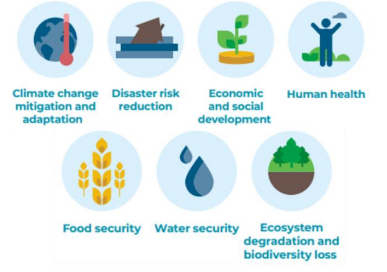
\includegraphics[width=0.50\linewidth]{figures/ThesevenNBSgoals.png}
%     \caption{Seven goals for achieving a good NBS}
%     \label{fig:placeholder}
% \end{figure}

\subsection{Design Plan}

Hier komt de procedure te staan hoe het design tot stand zal gaan komen en welke stappen gemaakt zullen worden. Uitleggen dat het een iteratief process is om de D te vinden doormiddel van de krachten en momentensom. De momentensom moet 0 zijn onderaan en hiermee kan dan de D bepaald worden. 

\subsection{Design}

\subsubsection{Problem Description}

Hier komt een schets van de situatie. Ook komen hier de parameters die nodig zijn bij het ontwerpen van een sheet pile.

\subsubsection{Soil Profile and Parameters}
To be able to design the sheetpile, the soil layers along with their geotechnical parameters should be known. In paragraph \ref{par:geology}, the geological background for the area of interest was given and this serves as the basis for deriving soil layers and parameters. The borehole in figure \ref{fig:borehole} is deemed the most relevant source. The borehole shows a top layer with fine/medium sands. Below, clay/clayey sand can be found, and the bottom layer consists of medium sand. This is in accordance with the geological profile that was provided before in figure \ref{fig:geolprofile}, which describes a transition from near-surface beach ridges, dunes, beach plains, and delta subaerial facies to deeper open estuaries and marine deposists. The top deposits help declare the presence of sandy deposits at the top of the borehole and the layers of clay/clayey sand below correspond to estuarine deposits. Finally, old marine/fluvial deposits were likely compacted and lead to the layer of medium sand found at the bottom of the borehole.

Because of the resemblance between the local borehole and the geological profile given before, the layering as shown in figure \ref{fig:borehole} is deemed representative for the whole study area. Based on this layering the relevant parameters can be derived, the result is shown in table \ref{tab:soil_layers}.

\begin{table}[H]
    \centering
    \begin{tabular}{|c|c|c|c|c|c|c|c|}
        \hline
        Start layer (m) & End layer (m) & Soil type & \makecell{ $\gamma_d$ \\ (kN/m$^3$) } & \makecell{ $\gamma_{sat}$ \\ (kN/m$^3$) } & \makecell{ $\varphi'$ \\ ($^\circ$) } & \makecell{ $c'$ \\ (kPa) } & \makecell{ $c_u$ \\ (kPa) } \\
        \hline
        0 & 2 & Fill (Topsoil/Agricultural) & 12 & 12 & 15 & 2.5 & 20 \\
        2 & 7 & Fine/medium sand & 17 & 19 & 30 & 0 & - \\
        7 & 10 & Clay & 14 & 14 & 17.5 & 0 & 25 \\
        10 & 15 & Clayey sand & 18 & 20 & 25 & 0 & - \\
        15 & 16 & Clay & 14 & 14 & 17.5 & 0 & 25 \\
        16 & 17.5 & Clayey sand & 18 & 20 & 25 & 0 & - \\
        17.5 & 32 & Medium sand & 18 & 20 & 32.5 & 0 & - \\
        \hline
    \end{tabular}
    \caption{Soil stratigraphy and geotechnical properties.}
    \label{tab:soil_layers}
\end{table}

The parameters in table \ref{tab:soil_layers} were derived from the Eurocode \autocite{stichtingkoninklijknederlandsnormalisatieinstituutNederlandseNormNEN2025}. Because of limited knowledge on soil characteristics, conservative estimates were made based on this code. In the borehole, no explicit information is given on the top fill layer. Therefore, conservative parameters were assumed based on typical values for organic topsoil.



Hier komt te staan wat de lengte en diepte van de sheet piles zullen worden. En welk profiel gebruikt zal worden voor de sheet piles. Ook de bepalende combinatie van rekenwaarde laten zien in een tabel.

\subsubsection{Loads}

Hier komt een beschrijving van de verschillende krachten die op de damwand komen te staan. Denk hierbij aan de earth pressure, water pressure en de golf energie force.

\subsubsection{Effective Stress}

Uitleg over hoe de effective stress berekend wordt met een afbeelding van de passive en active side en een tabel met de belangrijkste waarden. Uitleg dat alles onder de dredging line een waarden zal komen die uit een onbekende D zal bestaan.

\subsubsection{Hydrostatic Water Pressure}

Uitleg over hoe de hydrostatic water pressure berekend wordt met een afbeelding van de passive en active side en een tabel met de belangrijkste waarden. Uitleg dat alles onder de dredging line een waarden zal komen die uit een onbekende D zal bestaan.


\subsubsection{Earth Pressure}

Uitleg over hoe de active en passive earth pressure berekend wordt met een afbeelding en een tabel met de belangrijkste waarden. Uitleg dat alles onder de dredging line een waarden zal komen die uit een onbekende D zal bestaan. 

\subsubsection{Balance of Forces}

Vanuit de active en passive earth pressure de krachten kunnen bepalen doormiddel van vermenigvuldiging met de hoogte van de laag. Alle krachten laten zien in een tabel en ook een afbeelding van de krachten per driehoek en vierkant. Dit in de tabel mooi laten zien. Ook de balanssom van krachten beschrijven.

\subsubsection{Balance of Moments}

De momentensom om het laagste punt van de sheet pile gelijkstellen aan 0. Dit laten zien in een afbeelding en de uiteindelijke vergelijking die bestaat ui waardes en een onbekende D. Hieruit de wortel en d bepalen die de sheet pile zal moeten hebben. Ook een plaatje van de momenten lijn over de gehele damwand laten zien.

\subsection{Structural Verification}

\subsubsection{ULS and SLS}

\subsubsection{Normal Force}

\subsubsection{Moments}

\subsubsection{Deflection}

\subsection{Conclusion}

\section{Nature-based Solutions for dry sand mining}